\subsubsection{Аналитическая составляющая}
На сегодняшний день существует следующая классификация алгоритмов и протоколов
для распределёных реестров (Рис. \ref{2014protocol}):

\begin{figure}[h!]
    \centering
    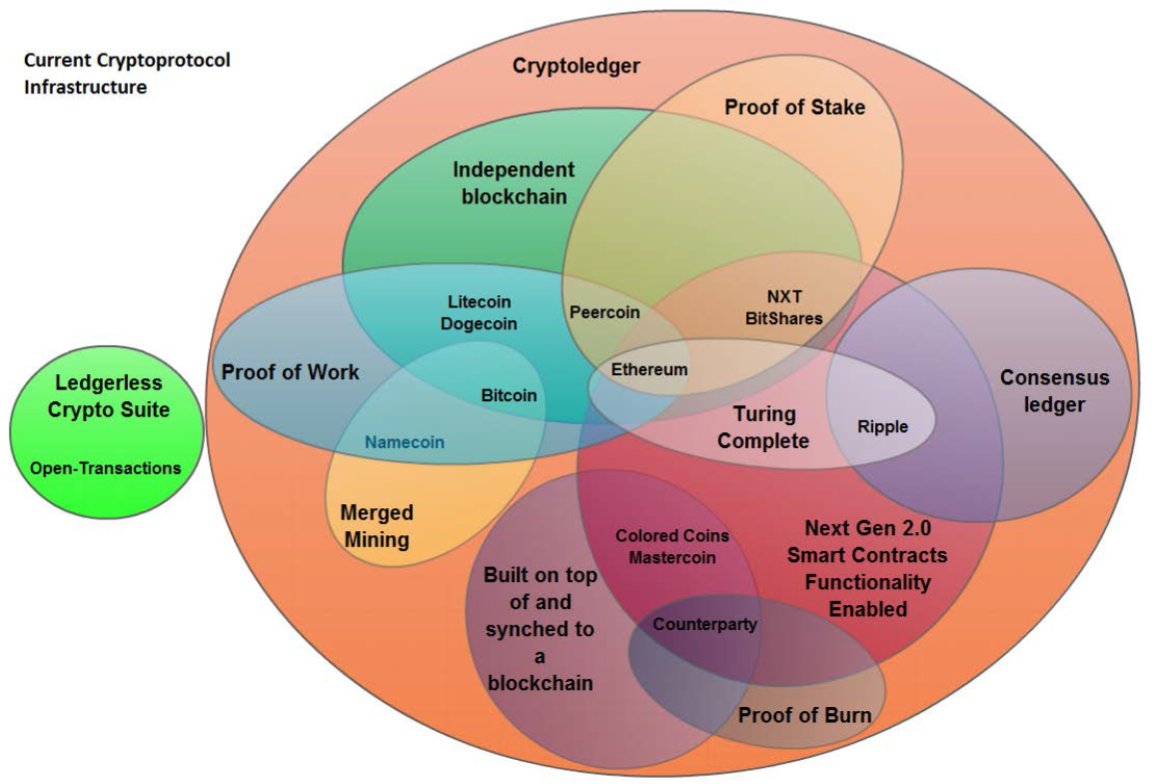
\includegraphics[width=0.8\textwidth]{./images/current_protocols}
    \caption{Классификация на 2014 год \cite{TimSwanson2014}}\label{2014protocol}
\end{figure}

Данная классификация представлена в книге Тима Суэнсона \cite{TimSwanson2014} и
являлась актуальным на 2014 год представлением классификации криптографических
алгоритмов и протоколов для распределённых реестров. Сегодня, когда появилось
множество новых алгоритмов и были изобретены уникальные типы реестров, данная
классификация утратила свою актуальность и нуждается в обновлении и
актуализации. В рамках данной работы будет представлена новая классификация
алгоритмов и протоколов для распределённых реестров. Классификация сохранит
принципы построения и представления своего предшественника.

\subsubsection{Программная составляющая}
\paragraph{Codecreator.com}
Данный ресурс \cite{CodeCreator} (на вкладке blockchain) представляет собой
сервис, предназначенный для развёртывания реестра на сервере Amazon AWS. Ресурс
позволяет развернуть реестры, основанные на Ethereum и Hyperledger. Ресурс
предназначен для крупных бизнес проектов, требующих рабочий код быстро. Имеет
бесплатную пробную версию.

\paragraph{Azure BaaS}
Данная платформа \cite{MicrosoftAzure}, Microsoft Azure Blockchain as a
Service, обеспечивает быструю, относительно недорогую, платформу для создания и
развертывания блокчейн-приложений. Azure предлагает Blockchain как сервис
(BaaS), а значит, встраивание кода блокчейна в код не предусматривается. Есть
поддержка самых популярных реестров, таких как Ethereum, Quorum, Hyperledger
Fabric, Corda.

\paragraph{Magic Code Generator}
Релиз данной платформы \cite{mcg} ещё не состоялся.  Документы, содержащиеся на
страницах описывают сервис, предназначенный для построения приложений,
взаимодействующих с сетями реестров. Например, онлайн биржу валют. Так же
сервис имеет возможность создания blockchain-based приложений.


Данный проект \emph{прямым} аналогом ни одного из приведённых приложений не
является. Это позволяет сказать, что проект уникальный в своём роде. Тем не
менее, есть сходства и различия, по которым можно привести следующее сравнение
(Табл. 1).

\begin{center}
    \begin{tabular}{ | p{4cm} | c | c | c | c | }
    \hline
    \hline
      Признак & Codecreator & Azure BaaS & MagicCodeGenerator\footnotemark & \textbf{GSL} \\ \hline
      Встраивание кода в своё приложение & Частично & Частично & --- & \textbf{Да} \\ \hline
      Моментальное развёртывание & --- & --- & --- & \textbf{Да} \\ \hline
      Вариаций алгоритмов использования & < 5 & < 10 & 0 & \textbf{24} \\ \hline
      Стоимость & $\approx$5600 руб./мес. & $\approx$3300 руб./мес. & Не известно & \textbf{0 руб. / мес.} \\ \hline
    \hline
  \end{tabular}

    \vspace{-5cm} \hfill \emph{Таблица 1. Сравнение с аналогами} \vspace{5cm}
\end{center}

\footnotetext{Релиз MagicCodeGenerator ещё не состоялся.}
